% THIS IS SIGPROC-SP.TEX - VERSION 3.1
% WORKS WITH V3.2SP OF ACM_PROC_ARTICLE-SP.CLS
% APRIL 2009
%
% It is an example file showing how to use the 'acm_proc_article-sp.cls' V3.2SP
% LaTeX2e document class file for Conference Proceedings submissions.
% ----------------------------------------------------------------------------------------------------------------
% This .tex file (and associated .cls V3.2SP) *DOES NOT* produce:
%       1) The Permission Statement
%       2) The Conference (location) Info information
%       3) The Copyright Line with ACM data
%       4) Page numbering
% ---------------------------------------------------------------------------------------------------------------
% It is an example which *does* use the .bib file (from which the .bbl file
% is produced).
% REMEMBER HOWEVER: After having produced the .bbl file,
% and prior to final submission,
% you need to 'insert'  your .bbl file into your source .tex file so as to provide
% ONE 'self-contained' source file.
%
% Questions regarding SIGS should be sent to
% Adrienne Griscti ---> griscti@acm.org
%
% Questions/suggestions regarding the guidelines, .tex and .cls files, etc. to
% Gerald Murray ---> murray@hq.acm.org
%
% For tracking purposes - this is V3.1SP - APRIL 2009

\documentclass{acm_proc_article-sp}
\usepackage{amsmath}
\usepackage{url}
\usepackage{tikz}
\usetikzlibrary{bayesnet}

\begin{document}

\title{A robust framework for estimating linguistic alignment in social media conversations\titlenote{Title note?}}
%\subtitle{[Extended Abstract]
%}
%
% You need the command \numberofauthors to handle the 'placement
% and alignment' of the authors beneath the title.
%
% For aesthetic reasons, we recommend 'three authors at a time'
% i.e. three 'name/affiliation blocks' be placed beneath the title.
%
% NOTE: You are NOT restricted in how many 'rows' of
% "name/affiliations" may appear. We just ask that you restrict
% the number of 'columns' to three.
%
% Because of the available 'opening page real-estate'
% we ask you to refrain from putting more than six authors
% (two rows with three columns) beneath the article title.
% More than six makes the first-page appear very cluttered indeed.
%
% Use the \alignauthor commands to handle the names
% and affiliations for an 'aesthetic maximum' of six authors.
% Add names, affiliations, addresses for
% the seventh etc. author(s) as the argument for the
% \additionalauthors command.
% These 'additional authors' will be output/set for you
% without further effort on your part as the last section in
% the body of your article BEFORE References or any Appendices.

\numberofauthors{3} %  in this sample file, there are a *total*
% of EIGHT authors. SIX appear on the 'first-page' (for formatting
% reasons) and the remaining two appear in the \additionalauthors section.
%
\author{
% You can go ahead and credit any number of authors here,
% e.g. one 'row of three' or two rows (consisting of one row of three
% and a second row of one, two or three).
%
% The command \alignauthor (no curly braces needed) should
% precede each author name, affiliation/snail-mail address and
% e-mail address. Additionally, tag each line of
% affiliation/address with \affaddr, and tag the
% e-mail address with \email.
%
% 1st. author
\alignauthor
Gabriel Doyle\\
       \affaddr{Department of Psychology}\\
       \affaddr{Stanford University}\\
       \affaddr{Stanford, CA 94305}\\
       \email{gdoyle@stanford.edu}
% 2nd. author
\alignauthor
Dan Yurovsky\\
       \affaddr{Department of Psychology}\\
       \affaddr{Stanford University}\\
       \affaddr{Stanford, CA 94305}\\
       \email{yurovsky@stanford.edu}
% 3rd. author
\alignauthor
Michael C. Frank\\
       \affaddr{Department of Psychology}\\
       \affaddr{Stanford University}\\
       \affaddr{Stanford, CA 94305}\\
       \email{mcfrank@stanford.edu}
}
% There's nothing stopping you putting the seventh, eighth, etc.
% author on the opening page (as the 'third row') but we ask,
% for aesthetic reasons that you place these 'additional authors'
% in the \additional authors block, viz.
%\additionalauthors{Additional authors: John Smith (The Th{\o}rv{\"a}ld Group,
%email: {\texttt{jsmith@affiliation.org}}) and Julius P.~Kumquat
%(The Kumquat Consortium, email: {\texttt{jpkumquat@consortium.net}}).}
%\date{30 July 1999}
% Just remember to make sure that the TOTAL number of authors
% is the number that will appear on the first page PLUS the
% number that will appear in the \additionalauthors section.

\maketitle
\begin{abstract}
%People tend to adopt behaviors similar to their conversational partners' behaviors, including similar postures, gestures, and language. Lexical alignment, an increased probability of using words that one's partner has used, has been studied in a range of conversational settings, but with little standardization in its measure. We propose a straightforward model-based approach to calculating linguistic alignment, with a focus on the sparse data observed in social networks.  We propose a set of desiderata for any measures of word-based alignment and show that this measure fulfills these desiderata on simulated data. We then use our measure to replicate an existing result on alignment on Twitter, and show that the measure's improved resolution reveals a previously undetectable effect of interpersonal power in social media interactions.

When people talk, they tend to adopt the behaviors, gestures, and language of their conversational partners. This ``accommodation'' to one's partners is largely automatic, but the degree to which it occurs is influenced by social factors, such as gender, relative power, and attraction. In settings where such social information is not known, this accommodation can be a useful cue for the missing information.  This is especially important in web-based communication, where social dynamics are often implicit and fluid.  But connecting accommodation and social dynamics on the web requires accurate quantification of the different amounts of accommodation being made. 

We focus specifically on accommodation in the form of ``linguistic alignment'': the amount that one person's word use is influenced by another's. Previous studies have used many measures for linguistic alignment, with no clear standard.  In this paper, we lay out a set of desiderata for a linguistic alignment measure, including robustness to sparse and short messages, explicit conditionality, and consistency across linguistic features with different baseline frequencies.  We propose a straightforward and flexible model-based framework for calculating linguistic alignment, with a focus on the sparse data and limited social information observed in social media.  We show that this alignment measure fulfills our desiderata on simulated data. We then use our measure to replicate an existing result on alignment on Twitter, and show that the measure's improved resolution reveals a previously undetectable effect of interpersonal power in social media interactions.

\end{abstract}

% A category with the (minimum) three required fields
\category{?.?}{Applied Computing}{Psychology}
\category{?.?}{Applied Computing}{Sociology}
\category{?.?}{Human-centered computing}{Social media}
\category{?.?}{Human-centered computing}{Social networks}

\terms{[TODO: replace with the terms I used in the submission form]}

%\keywords{ACM proceedings, \LaTeX, text tagging} % NOT required for Proceedings

\section{Introduction}

When people interact, they tend to act similarly, adopting similar postures, speaking in similar ways, and using similar words. Such changes, which can be grouped under the general term \textit{communication accommodation} \cite{GilesCouplandCoupland1991}, are a pervasive part of human interactive behavior. Accommodation arises in many different dimensions of interaction, including gesture, posture, tone, and language use \cite{CondonOgston1967,BourhisGiles1977,GilesSchererTaylor1979,LeveltKelter1982,HaleBurgoon1984,ChartrandvanBaaren2009}. From a scientific perspective, greater degrees of accommodation can signal power relationships or affiliation \cite{WillemynsEtAl1997,Gnisci2005,DNMEtAl2012}, and from an engineering perspective, interactive agents that accommodate are seen as friendlier and more human \cite{NassLee2000}. 

Thus, the phenomenon of accommodation has important implications for many fields, and one of the most important and well-studied forms of accommodation is \textit{linguistic alignment}, in which conversational partners align aspects of their communicative style and content to one another. Roughly speaking, linguistic alignment can be measured as the change in likelihood of using a given ``marker'' -- most often a word (e.g., \textit{you}) or word category (e.g., prepositions) -- based on its use by a partner. 

But while the basic idea of linguistic alignment has been used in a range of studies across fields, it has been quantified using a variety of substantially different measures \cite{IrelandEtAl2011,DNMGamonDumais2011,FusaroliEtAl2012}. Some measures conflate influences that others separate; some combine features that others do not; and some account for individual speaker differences that others do not. In addition, there is fairly limited research into how appropriate these measures are for different types of data, such as the sparse interactional data of social media and other web-based settings (though see \cite{XuReitter2015}).  

Our goal in this paper is to address this issue. To do so, we begin by describing a set of desiderata for linguistic alignment measures. We then report simulations showing that existing measures of alignment fail when faced with sparse linguistic data of the type that are common on the web. We propose a new model-based alignment metric and show that it fulfills our desiderata. We end by testing this new model using Twitter data and show that it succeeds in detecting the the influence of power dynamics on accommodation behavior where one previous metric failed. 

\section{Prior work on Accommodation and Alignment}

Accommodation generally is a deeply-ingrained human behavior.  Children as young as 12 months old accommodate to their parents on pitch \cite{Lieberman1967}, and fictional dialogues show similar alignment to real ones. These two datapoints suggest that accommodation is a crucial and ``unmediated'' mechanism \cite{PickeringGarrod2004,DNMLee2011}.  Accommodation can even influence human-computer interactions, with people rating interactions with accommodating computer systems as more satisfying even when the conversant is known to be a computer \cite{NassLee2000,vanBaarenEtAl2003,BraniganEtAl2010}.

Linguistic accommodation, which we distinguish here by referring to it as \emph{alignment}, has been one of the key domains in which hypotheses about accommodation have been tested. A major branch of this work is known as Linguistic Style Matching (LSM) \cite{NiederhofferPennebaker2002,IrelandEtAl2011}.  The focus of LSM is on ``stylistic'' accommodation, as opposed to content accommodation; practically, LSM examines the reuse of function words (prepositions, pronouns, articles, etc.) that carry little inherent semantic information, as opposed to content words (nouns, verbs, etc.). This focus on function words is motivated by the argument that function words represent a stylistic choice, as a speaker can choose between many different function words in composing a message, without substantially changing the meaning of the message.  Function word use has been shown to vary between people but to remain fairly consistent within a single person's writing \cite{PennebakerKing1999}. As such, it has been fruitfully applied to authorship attribution as well \cite{boyd2015}. \footnote{This interest in function words over content words is effectively the mirror image of many document classification methods, such as topic models \cite{BleiNgJordan2003}, which focus on content word co-occurrences and typically \emph{exclude} function words.}

Accommodation, especially linguistic alignment, can be a critical part of achieving social goals.  Performance in a variety of cooperative decision-making tasks has been positively related to the participants' linguistic convergence \cite{FusaroliEtAl2012,KacewiczEtAl2013}.  Match-matching in speed dating as well as stability in established relationships have been linked to increased alignment \cite{IrelandEtAl2011}.  Alignment can also improve persuasiveness, encouraging listeners to follow good health practices \cite{KlineCeropski1984} or convincing children to share more \cite{BurlesonFennelly1981}.

Alignment typically is convergent, making the conversants more similar, but the degree and direction of alignment differs from situation to situation. In some situations people may diverge, intentionally or not; this divergence is often tied to a particular social goal, such as maintaining an appropriate power dynamic between doctors and patients \cite{Ferrara1991}. In addition, different dimensions or features may exhibit convergence at different strengths \cite{ThakerarGilesCheshire1982,BilousKrauss1988,DNMGamonDumais2011} and/or different time-scales \cite{Ferrara1991}.  Lastly, alignment and accommodation are usually incomplete, in that people become more similar but not the same; \cite{GilesCouplandCoupland1991,GilesSmith1979} show that near-complete accommodation can come off as cloying or derisive.

Variability in accommodation behavior can be sociologically and psychologically meaningful.  Power relationships are an important source of differential accommodation, with less powerful conversants generally accommodating more to more powerful conversants than vice versa. Prominent examples of such asymmetric accommodation include interviews and jury trials \cite{WillemynsEtAl1997,Gnisci2005,DNMEtAl2012}.  Additionally, factors such as gender, likability, respect, and attraction all interact with the magnitude of accommodation \cite{BilousKrauss1988,Natale1975}. Such differences in accommodation can also be indicative of changes to the power dynamic: In U.S. Supreme Court transcripts, \cite{guo2015} showed that depending on the accommodation dimension, justices -- who are more powerful by any intuitive assessment -- may nevertheless accommodate more to lawyers, perhaps because the lawyers have the local power to answer justices' questions.

Accommodation can also be a critical part of achieving social goals.  Performance in a cooperative decision-making task was positively related to the participants' linguistic alignment \cite{FusaroliEtAl2012}.  Match-matching in speed dating as well as stability in established relationships have been linked to more similar language use \cite{IrelandEtAl2011}.  Accommodation can also improve persuasiveness, encouraging listeners to follow good health practices \cite{KlineCeropski1984} or convincing children to share more \cite{BurlesonFennelly1981}.

% \subsection{Linguistic Alignment}


%Discuss previous work showing that alignment can be indicative of important sociological/demographic variables. Provide some quick examples of linguistic accommodation being predictive of outcomes in, for example, cooperative tasks to suggest that there are important applications for this paper. 

%Brief overview of the critical problem: while there are a lot of promising results suggesting this is important, there are no standard measures being employed, and that these may measure different things. There is a need to think carefully about what we do and don't want to measure, a need to account for individual differences, and a need to be robust to the often sparse data that (especially web-based) interactions often provide.

\section{Desiderata for Measures of Linguistic Alignment }

Accommodation and related concepts have been approached from many different fields of study, leading to many different approaches to quantifying linguistic alignment. On one hand, this is a helpful proliferation. Alignment must be a very robust characteristic of human socialization if its effects appear using so many different estimation methods.  On the other hand, measures used in different studies are difficult to compare, and some studies separate factors that other conflate. From the perspective of standardization and comparison, a single measure would allow further theoretical progress. But what measure to select? 

In what follows, we propose a set of desiderata for linguistic alignment measures. At the highest level, the goal of a measure of linguistic alignment should be to quantify the amount that one person's language use is influenced by another's: We are interested in seeing how much a person changes when speaking to different people, and to what extent such changes increase the similarity between the speakers. Also, because linguistic alignment can, in principle, be measured on many different words and categories, we want a measure that can be compared across linguistic features with very different frequencies.  Furthermore, because different features may align differently \cite{BilousKrauss1988,Ferrara1991}, we want a measure that is flexible enough to account for these differences. Although previous desiderata have been proposed \cite{XuReitter2015}, these requirements are focused towards theoretical goals (e.g., consistency across different structural levels). Such goals are important, but presuppose basic statistical properties like a lack of bias when estimated for markers at different frequencies. Our concern here is with establishing these more basic statistical desiderata. 

% [TODO: fomralize the alignment problem]

\subsection{Conditionality and baselining} 

An alignment measure must provide a measure of directional linguistic influence, not just general similarity. In addition, many existing measures fail to account for the possibility that speakers may already be very similar before they start talking.  One example of the importance of conditionality is \cite{IrelandEtAl2011}, who show that speed daters with more similar word distributions are more likely to form a connection, but do not control for how similar the speed daters' language use is independent of each other.  It may be that some people happen to speak more similarly from the start, rather than accommodating each other, and that this inherent similarity is making them a more likely couple.

The relevant theoretical distinction is between \textit{accommodation} and \textit{homophily}.  If two people speak in a similar manner, it may be that they have \emph{observed} each other's style of speech and have aligned to each other (accommodation) \cite{DNMGamonDumais2011}. However, it also may be that these two people happen to have \emph{inherently similar} speaking styles, perhaps because they have similar linguistic backgrounds or similar linguistic pressures (homophily). Accommodation and homophily are likely to have similar effects on outcome measures such as comprehension, likability, and task success, based on similarity-attraction theories, but differ substantially in terms of their theoretical import \cite{Byrne1969,Triandis1960,GilesSmith1979}.  

Conditionality is perhaps the most critical desideratum for a measure of alignment: without it, any result may be due to mere homophily. To address this issue, when calculating alignment Danescu-Niculescu-Mizil and colleagues \cite{DNMGamonDumais2011,DNMLee2011,DNMEtAl2012} subtract off a speaker's average frequency of using a linguistic marker. The Hierarchical Alignment Model we present here represents an extension of their measure to satisfy our full set of dseiderata. 

% One major goal for an alignment measure is thus to decouple these influences to see if they have independent effects.  Meeting this goal would also the measure to detect asymmetries in alignment, in which one speaker aligns more than the other, which is important for investigating sociological influences on alignment \cite{DNMEtAl2012}.

\subsection{Separability across markers}

Accommodation is not a monolithic process; people may converge on some dimensions while diverging on others \cite{BilousKrauss1988,Ferrara1991}. In fact, similarly high levels of accommodation on multiple dimensions may even be counter-productive, giving the impression of mocking or condescending to the audience \cite{GilesSmith1979,GilesCouplandCoupland1991}. Empirically, for specifically linguistic alignment, different markers may have distinctly different alignments \cite{DNMGamonDumais2011,IrelandEtAl2011}. For instance, \textit{I} and \textit{we} usage is likely to converge between speakers, but \textit{you} usage is likely to diverge \cite{NiederhofferPennebaker2002,GonzalesHancockPennebaker2010}. These differences can have important implications for applications of alignment; \cite{FusaroliEtAl2012} found that increased alignment on expressions of confidence improved group performance in a task, but across-the-board increases in alignment \emph{reduced} group performance.  As such, we want a measure that can estimate different alignment values for different markers, with the possible option of aggregating over markers when needed.

\subsection{Consistency across marker frequencies} 

Different words have radically different baseline frequencies: a few words are used very often, but the bulk of our vocabularies are rarely used. As discussed above, it is undesirable to aggregate alignment values across markers, but consistency in our alignment measure is important if we want to investigate how (or whether) baseline frequencies interact with alignment.
% \footnote{For example, \cite{Church2000} use a non-parametric measure of burstiness, similar to a within-document alignment measure, to show that the effect on burstiness of word class was an order of magnitude greater than the effect of baseline frequency.}   
As such, we want a measure for which alignment effect strengths are not significantly biased by baseline word frequencies. To assess measures on this desideratum, we will test potential alignment measures against simulated data with known alignment strengths and marker frequencies to ensure comparability across a wide range of marker frequencies.  %This is one desideratum that motivates differences between our model and the DNM measure.

\subsection{Robustness to sparse data} 

Much work on communication accommodation and linguistic alignment, especially early work, focused on cases where a small set of people interact extensively, allowing accommodation effects to be estimated from a fairly large dataset \cite{Ferrara1991,GonzalesHancockPennebaker2010,IrelandEtAl2011}.  In many applications, especially those on the Web, however, datasets have the opposite character: a large number of people interact briefly and data about any given interaction is sparse. For example, in the Twitter dataset we examine here, many of our interacting pairs exchange only two messages, containing a maximum of 280 characters. These passing interactions may be importantly different from repeated interactions with close friends.  Our measures must be robust enough to extract accurate alignment values from these sparse interactions, so that they can be compared against estimates from more extensive interactions.  

\section{Existing Measures for Linguistic Alignment}
An extensive range of measures have been used in the alignment literature. Rather than representing a comprehensive review, this section provides a sampling of some influential measurement methods, and discusses how they fit the desiderata described above.  

% A summary of the measures' performance on the desiderata is given in Table \ref{tab:desiderata}. 

\subsection{Subtractive Conditional Probability (SCP)} 

Danescu-Niculescu-Mizil and colleagues \cite{DNMGamonDumais2011} presented a subtractive conditional probability measure, capturing the increase in the conditional probability of using a marker, given that it has been used by a conversational partner.  Consider a set of messages from speaker $a$ that each gets a reply from speaker $b$.  Let $A$ indicate that $a$ used the marker in a message, and $B$ indicate that $b$ used the marker in a reply.  Then the subtractive conditional probability alignment score is:

\begin{equation}
Align_{SCP} = p(B|A) - p(B)
\end{equation}

This measure satisfies the conditionality/baselining condition because the alignment estimate takes into account how much more likely $b$ is to use the marker in response to $a$ than some baseline.\footnote{The computation of this baseline could be questioned, however; \cite{DNMGamonDumais2011} limit the calculation of $p(B)$ to the conversations between $a$ and $b$, not all of $b$'s conversations.}  In addition, SCP is calculated independently for each marker, so it meets the marker separability criterion.  It is the only existing measure we will look at that satisfies both of these desiderata.

It fails on the marker comparability criterion, however.  First, the range of possible alignment values for SCP depends on the baseline $p(B)$, with the alignment estimate falling in the interval $[-p(B),1-p(B)]$.  In addition, $p(B) = p(B|A)p(A) + p(B|\neg A)p(\neg A)$, making the alignment range also dependent on $p(A)$:

\begin{align*}
Align_{DNM} & = & p(B|A) - (p(B|A)p(A) + p(B|\neg A)p(\neg A)) \\
& = & (1-p(A))(p(B|A) - p(B|\neg A)
\end{align*} 

This means that the range of the DNM alignment estimate for a given marker is the intersection of the intervals $[-p(B), 1-p(B)]$ and $[2(p(A)-1), 2(1-p(A))]$, making the direct comparison of alignment on markers with different baseline frequencies difficult; this point is illustrated through simulations in Section \ref{sec:simulations}.  Lastly SCP has been applied only to conversations with at least 10 messages in previous work; we investigate its robustness to sparse data below.
% Lastly, the DNM measure may not be robust to sparse data, as it has been applied only to conversations with at least 10 messages in previous work.  In tests on our simulated data, we find that removing this restriction does not appear to affect the results on our simulated data substantially; as such, we report results without the cutoff. It may be necessary in other cases.

\subsection{Local Linguistic Alignment (LLA)} 

\textit{local linguistic alignment} (LLA) is originally proposed by \cite{FusaroliEtAl2012}; we use the formalization from \cite{WangReitterYen2014}.  Suppose $a$ sends message $M_a$ to $b$, who replies with $M_b$. Then:

\begin{equation}
Align_{LLA} = \frac{\sum_{w_i \in M_b} \delta(w_i \in M_a)}{length(M_a)length(M_b)}
\end{equation}

Intuitively, LLA is the percentage of words in the reply that also appeared in the first message, divided by the length of the first message.  This fulfills half of the conditionality/baselining desiderata; the numerator is a conditional distribution, only counting words that have been repeated in the reply.  But no baselining is being done to separate homophily from alignment; If two speakers happen to have similar vocabulary distributions, they can end up with high LLA values without accommodating each other at all.

Because LLA does not meet the baselining desideratum, we mention performance on other desiderata only briefly. Discriminate LLA, where only words from a particular category are counted, meets the marker separability desideratum.  Indiscriminate LLA, which counts all words, does not meet this desideratum, and \cite{FusaroliEtAl2012} show opposite alignment effects on task performance depending on whether the disparate markers are treated separately or lumped together.  For these reasons, we only test discriminate LLA in our simulations. Discriminate LLA is also not consistent across different message lengths, as the maximum value of the numerator is $length(M_b)$, meaning that the LLA value is bounded above by $length(M_a)$. Replies to short messages, then, have higher maximum LLA values than replies to long messages.

% \footnote{We do not consider 

%  [TODO: add a footnote in here that XuReitter2015 compared LLA and SCC and found LLA better, so we won't consider SCC here.]

\subsection{Linguistic Style Matching (LSM)} 

A great deal of the work on linguistic alignment from a psychological perspective comes from Pennebaker and colleagues \cite{NiederhofferPennebaker2002,GonzalesHancockPennebaker2010,IrelandEtAl2011}, including the Linguistic Inquiry and Word Count system that we use below to establish our marker categories \cite{LIWC}.  The alignment measure used in this work is Linguistic Style Matching (LSM). As with the SCP measure, suppose we have a set of messages exchanged between $a$ and $b$, and $A$ (or $B$) indicates that $a$ (or $b$) has used the marker. Then LSM is defined as:

\begin{equation}
Align_{LSM} = 1 - \frac{|p(A)-p(B)|}{p(A)+p(B)}
\end{equation}

This measure does not meet the conditionality/baseline desideratum. Suppose $b$ used the marker only when $a$ did not, and never used it when $a$ did, and $a$ used the marker in about half of the messages, ignoring what $b$ was doing.  The intuitive sense of alignment is that $b$ is being divergent, and should have a large negative alignment score, while $a$ is simply not aligning at all. However, given that $p(A) \approx p(B) \approx 0.5$, the LSM for this pair would be near a perfect 1.  In addition, if two speakers have similar inherent distributions but diverge while talking to each other, they could have a much higher LSM score than two people with very dissimilar inherent distributions who align substantially. LSM fits the marker separability desideratum, as it is independently calculated for each marker; we show its performance on low-frequency markers and sparse data below. 
% Also, it is likely to have trouble with sparse language data as sparsity will add noise to the estimates of $p(A)$ and $p(B)$.

%\paragraph{Comparisons} Because we are only interested in alignment measures that meet the conditionality/baseline criterion, we will only be directly testing the DNM measure 

%\paragraph{Zelig Quotient}  

%\paragraph{Correlation?}

%\paragraph{Repetition Decay} These are good methods, but they're not exactly looking at our problem. Overview of Bayesian Echo Chamber since our measure is sort of a stripped-down version of it.

\section{Hierarchical Alignment Model}

\begin{figure*}[t]
  \begin{center}
    % model_lda.tex
%
% Copyright (C) 2010,2011 Laura Dietz
% Copyright (C) 2012 Jaakko Luttinen
%
% This file may be distributed and/or modified
%
% 1. under the LaTeX Project Public License and/or
% 2. under the GNU General Public License.
%
% See the files LICENSE_LPPL and LICENSE_GPL for more details.

% Latent Diriclet allocation model

%\beginpgfgraphicnamed{model-lda}
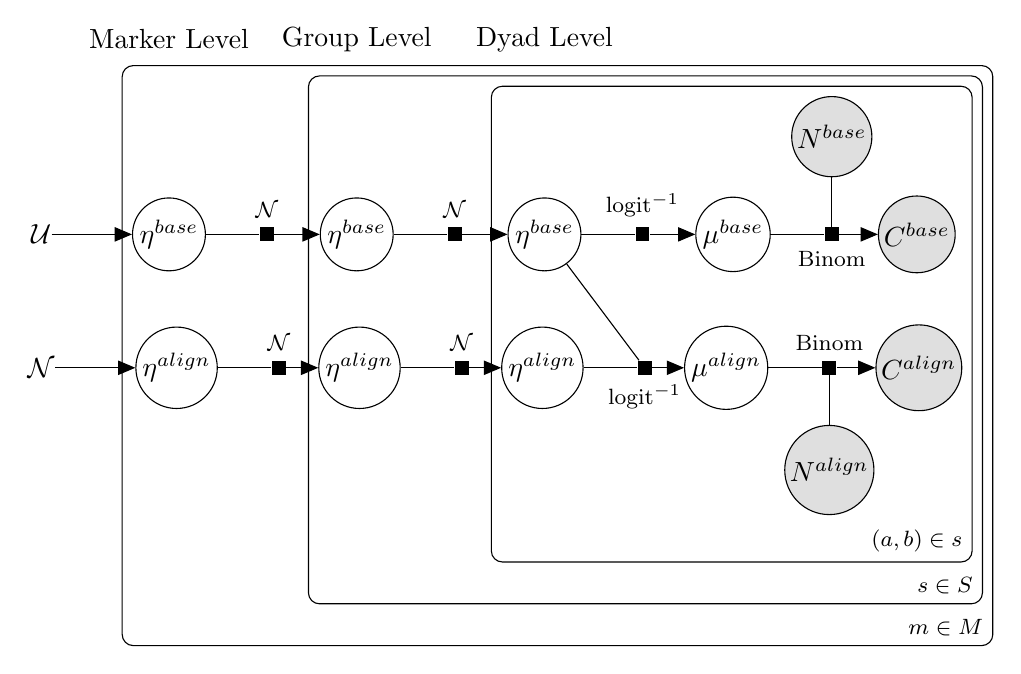
\begin{tikzpicture}[x=1.7cm,y=1.8cm]

  % Nodes

  \node[const] (base) {$\mathcal{U}$};
%  \node[latent,right=.6 of base] (n_b_m) {$\eta^{base}_m$}; 
%  \node[latent,right=.8 of n_b_m] (n_b_ms) {$\eta^{base}_{m,s}$};
%  \node[latent,right=.8 of n_b_ms] (n_b_mab) {$\eta^{base}_{m,a,b}$};
%  \node[latent,right=.8 of n_b_mab] (m_b_mab) {$\mu^{base}_{m,a,b}$};
%  \node[obs,right=.8 of m_b_mab] (C_b_mab) {$C^{base}_{m,a,b}$};

  \node[const,below=.8 of base] (align) {$\mathcal{N}$};
% \node[latent,right=.6 of align] (n_a_m) {$\eta^{align}_m$}; 
% \node[latent,right=.75 of n_a_m] (n_a_ms) {$\eta^{align}_{m,s}$};
% \node[latent,right=.75 of n_a_ms] (n_a_mab) {$\eta^{align}_{m,a,b}$};
% \node[latent,right=.75 of n_a_mab] (m_a_mab) {$\mu^{align}_{m,a,b}$};
% \node[obs,right=.8 of m_a_mab] (C_a_mab) {$C^{align}_{m,a,b}$};

  \node[latent,right=.6 of base] (n_b_m) {$\eta^{base}$}; 
  \node[latent,right=.85 of n_b_m] (n_b_ms) {$\eta^{base}$};
  \node[latent,right=.85 of n_b_ms] (n_b_mab) {$\eta^{base}$};
  \node[latent,right=.85 of n_b_mab] (m_b_mab) {$\mu^{base}$};
  \node[obs,right=.8 of m_b_mab] (C_b_mab) {$C^{base}$};

  \node[latent,right=.6 of align] (n_a_m) {$\eta^{align}$}; 
  \node[latent,right=.75 of n_a_m] (n_a_ms) {$\eta^{align}$};
  \node[latent,right=.75 of n_a_ms] (n_a_mab) {$\eta^{align}$};
  \node[latent,right=.75 of n_a_mab] (m_a_mab) {$\mu^{align}$};
  \node[obs,right=.8 of m_a_mab] (C_a_mab) {$C^{align}$};

  
  \node[const,above=1.05 of n_b_m] (marker) {Marker Level};
  \node[const,above=1.02 of n_b_ms] (group) {Group Level};
  \node[const,above=1.02 of n_b_mab] (dyad) {Dyad Level};

  % Factors
  
  \factor[right=of n_b_m] {n_b_m_f} {above:$\mathcal{N}$} {} {};
  \factor[right=of n_b_ms] {n_b_ms_f} {above:$\mathcal{N}$} {} {};
  \factor[right=of n_b_mab] {n_b_mab_f} {above:$\textrm{logit}^{-1}$} {} {};
  \factor[right=of m_b_mab] {m_b_mab_f} {below:Binom} {} {};

  \factor[right=of n_a_m] {n_a_m_f} {above:$\mathcal{N}$} {} {};
  \factor[right=of n_a_ms] {n_a_ms_f} {above:$\mathcal{N}$} {} {};
  \factor[right=of n_a_mab] {n_a_mab_f} {below:$\textrm{logit}^{-1}$} {} {};
  \factor[right=of m_a_mab] {m_a_mab_f} {above:Binom} {} {};

  %\factor[right=of C_b_mab] {C_b_mab_f} {above:Binom$} {} {};
  
  %\factor[above=of X]     {X-f}     {Multi} {} {} ; %
  %\factor[above=of T]     {T-f}     {left:Multi} {} {} ; %
  %\factor[above=of theta] {theta-f} {left:Dir} {} {} ; %

  % More nodes
  %\node[latent, right=of X-f] (phi)  {$\phi$}; %
  %\node[const, above=of phi]  (aphi) {$\alpha_\phi$}; %

  %\factor[above=of phi] {phi-f} {right:Dir} {} {} ; %

%  \node[obs,above=.35 of m_b_mab_f] (N_b_mab) {$N^{base}_{m,a,b}$};
%  \node[obs,below=.35 of m_a_mab_f] (N_a_mab) {$N^{align}_{m,a,b}$};

  \node[obs,above=.35 of m_b_mab_f] (N_b_mab) {$N^{base}$};
  \node[obs,below=.35 of m_a_mab_f] (N_a_mab) {$N^{align}$};


  \edge{base}{n_b_m};
  \factoredge {n_b_m}  {n_b_m_f}     {n_b_ms} ; %
  \factoredge {n_b_ms}  {n_b_ms_f}     {n_b_mab} ; %
  \factoredge {n_b_mab}  {n_b_mab_f}     {m_b_mab} ; %
  \factoredge {m_b_mab,N_b_mab} {m_b_mab_f} {C_b_mab}; %
 
   \edge{align}{n_a_m};
  \factoredge {n_a_m}  {n_a_m_f}     {n_a_ms} ; %
  \factoredge {n_a_ms}  {n_a_ms_f}     {n_a_mab} ; %
  \factoredge {n_a_mab,n_b_mab}  {n_a_mab_f}     {m_a_mab} ; %
  \factoredge {m_a_mab,N_a_mab} {m_a_mab_f} {C_a_mab}; %
 %\factoredge {atheta} {theta-f} {theta} ; %
  %\factoredge {phi}    {X-f}     {X} ; %
  %\factoredge {aphi}   {phi-f}   {phi} ; %

  %\gate {X-gate} {(X-f)(X-f-caption)} {T}

  \plate {pairplate} { %
    (N_b_mab)(C_b_mab) %
    (m_b_mab)(n_b_mab) %
    (N_a_mab)(C_a_mab) %
    (m_a_mab)(n_a_mab) %
  } {$(a,b) \in s$}; %
  \plate {subpopplate} { %
    (pairplate) %
    (n_b_ms) (n_a_ms) %
  } {$s \in S$} ; %
  \plate {} { %
    (subpopplate) %
    (n_b_m) (n_a_m)
  } {$m \in M$} ; %

\end{tikzpicture}
%\endpgfgraphicnamed

%%% Local Variables: 
%%% mode: tex-pdf
%%% TeX-master: "example"
%%% End: 

  \end{center}
  \caption{The Hierarchical Alignment Model (HAM). A chain of normal distributions generates a linear predictor $\eta$, which is converted into a probability $\mu$ for binomial draws of marker presence/absence.}\label{fig:model}
\end{figure*}

\subsection{Motivation}

Building on the probabilistic intuition motivating the SCP measure, we propose a Hierarchical Alignment Model (HAM). Specifically, our goal is to use model-based estimation of conditional probabilities to create a measure that is consistent across different marker frequencies and robustness to sparse data.  

To handle large baseline differences in marker frequency, we change the form of our alignment estimate from an additive effect in probability space to an additive effect in log-odds space. Having alignment as an additive effect in probability space means that the range of possible alignment strengths moves with the baseline; a more frequent marker can not show as much convergence as a less frequent marker can. If alignment is a linear effect in log-odds space, then alignment is defined in the range $(-\infty,+\infty)$ and is freed from the biasing influence of baseline probability, since even high probabilities can increase by large amounts in log-odds space.

To improve performance on sparse data we introduce a hierarchical prior on alignment values, parameterized by both marker and dyad (speaker/replier pair). In doing so, we introduce an assumption that, unless the data argues strongly otherwise, dyads are likely to have similar alignment behaviors on a given marker. This leads to more accurate estimates of marker frequency and alignment in sparse data dyads, since they are influenced by the alignment found in the dataset as a whole. This kind of hierarchical regularization has proven extremely valuable in a wide variety of applications \cite{gelman2006}.  

\subsection{Model}

We begin by conceptualizing a conversation as a tree; each message, aside from the first, is in response to a particular preceding message, but a message may elicit multiple replies. Tweets already fit this structure, because Twitter replies explicitly include which tweet a reply is directed to.  In settings without explicit reply structure, a message can be treated as a reply to all messages that came before it \cite{WangReitterYen2014} or thread reconstruction can be used to find individual reply links \cite{JonesEtAl2014}.

Suppose we observe a conversation that starts with Alice, who says ``hi.'' Bob replies to this message with ``hello there,'' and Alice responds with ``how are you?''. In addition, Eve jumps into the conversation by replying to Bob (``hi Bob!''). This conversation provides three message pairs:

\begin{align*}
[(A, \textrm{hi}), & (B: \textrm{hello there})] \\
[(B: \textrm{hello there}), & (A: \textrm{how are you?})] \\
[(B: \textrm{hello there}), & (E: \textrm{hi Bob}!)] 
\end{align*}

Following \cite{DNMGamonDumais2011}, we treat messages as binary vectors over words, rather than probability distributions or counts over words.  Because these are conversational messages, they tend to be short -- in the particular case of Twitter, messages contain on average approximately 3 to 6 markers---and thus this binarization instead of a count is not a severe simplification.\footnote{In fact, the shortness of the messages could introduce substantial noise via normalization within tweets, reducing robustness to sparse data.}  Alignment then is an increase in the probability of seeing a given marker (or marker category) in the second message of a pair given that it appeared in the first message of that pair.

Figure \label{fig:model} gives our graphical model for alignment. We treat pairs where the first message did contain the marker separately from those where the first message did not contain the marker.  The number of message pairs between a dyad of speakers $(a,b)$ is split into $N^{base}_{m,a,b}$, the number of pairs where $a$ did use the marker $m$, and $N^{align}_{m,a,b}$, the number of pairs where $a$ did not use $m$.  We also calculate the count of message pairs where the replier $b$ used the marker $m$ when $a$ did not ($C^{base}_{m,a,b}$) and when $a$ did ($C^{align}_{m,a,b}$).   These counts are assumed to come from binomial draws with probability $\mu^{base}$ or $\mu^{align}$.  These $\mu$ values are generated from the $\eta$ values in log-odds space by an inverse-logit transform, similar to linear predictors in logistic regression.

We implement alignment on these $\eta$ values; the $\eta^{base}$ variables are representations of the baseline frequency of a marker in log-odds space, and $\mu^{base}$ is simply a conversion of $\eta^{base}$ to probability space, the equivalent of an intercept term in a logistic regression. $\eta^{align}$ is an additive value, with $\mu^{align} = \textrm{logit}^{-1}(\eta^{base}+\eta^{align})$, the equivalent of a binary feature coefficient in a logistic regression.  Alignment is the change in log-odds of the replier using $m$ above their baseline usage of the marker. %Add footnote about lack of explicit negative influence of not using a word? If so, cite Chruch 2000 as reason -- orders of magnitude less.

Going up the hierarchy, the prior on the $\eta$ values has $\eta$ values specific to each marker-dyad combination, from which the $\mu$ values are calculated. One level above this are $\eta$ values for marker-group combinations. ``Group'' here is an intentionally vague classifier for groups of dyads.  In the present work, we divide dyads into groups based on the power differential in the dyad, but group divisions based on gender, conversation role, or any other variables are equally possible. This layer may also be omitted in cases where no group effects are being studied.

Lastly, there are $\eta$ values at the marker level, shared across all groups.  For $\eta^{align}$, this is a normal distribution centered at 0, biasing the model equally in favor of positive and negative alignments. For $\eta^{base}$, the overall frequency of a marker, we set the prior on this highest level parameter to be an uninformative uniform distribution over $[-5,5]$, as there is no strong reason to expect one particular marker frequency over another.  This range was chosen for convenience; it translates to approximately $[.006, .993]$ in probability space, which is well beyond the $[0.1,0.6]$ range of marker frequencies considered here.\footnote{While in principle an unbounded distribution is appropriate, \cite{GelmanEtAl2008} discuss the $[-5,5]$ interval for logistic regression coefficients as capturing likely coefficients; for modeling markers with very high or low probabilities, the Cauchy distribution recommended in that paper could replace the uniform distribution, allowing (rare) extreme $\eta^{base}$ values.}  Each layer of the $\eta$ parameters is generated by a normal distribution with variance $\sigma^2$.

\subsection{Model Fitting and Inference}

Alignment measures can be extracted from multiple different levels of this model hierarchy; we focus on the $\eta^{align}_{m,s}$ parameter, which is a single value estimating the mean alignment by dyads within a subpopulation. This value represents the change in the log-odds of using $m$ when replying to someone who has already used it, which constitutes our operationalization of alignment.

We implemented this model in RStan \cite{Stan}, with code available at \url{http://github.com/langcog/alignment}. The model is fit with 200 iterations of the sampler (100 discarded as burn-in) for each dataset; judging from trace plots, this setting led to reliable convergence.  We then extracted alignment estimates from each of the final 100 iterations of the model, and we report the 95\% highest posterior density interval on the parameter values in these plots.

% We suppose that different speakers and repliers may have different baseline usages.\footnote{This is an important assumption, as work in authorship attribution has found consistent and distinctive by-person usage rates for many of the function words that we use as markers.\cite{?}} This can be implemented either at the level of individuals or at a subpopulation level, with the subpopulations defined by sociologically relevant features (in our test case, verification status on Twitter). These values are implemented in logit space so that they can be defined over $ [-\infty,+\infty] $ and converted to probabilities using the inverse logit function. These subpopulation usage values are in turn drawn independently for each marker, as different markers may have different baseline rates or different alignment rates.  Finally, means for each marker over the population as a whole are drawn from a normal distribution that serves primarily as a regularizer.  [TODO: probably swap order to start with hgihest-level draw and work down to individuals.]

%Our focus is on alignment, the change in a marker's probability when the preceding message has used that marker versus when it has not.  There are potentially many ways of calculating this change; we break from the subtrcative conditional probability measure and 

\section{Experiment 1: Simulations}
\label{sec:simulations}

We begin by testing the HAM model for consistency across different marker frequencies and robustness to sparse data.  We report the results of two simulations: the first generates alignment on a per-message basis (more like the SCP/HAM measures' assumptions), and the second generates alignment on a per-word basis (presumably more similar to actual production).  We show greater consistency and more accurate alignment estimates for the HAM model over the existing measures in both cases.

\subsection{Simulation 1: Per-message Alignment}

Our first simulation uses a simple generative model that treats the presence or absence of a marker in a message as the relevant quantity. Instead of attempting to estimate word productions based on unigram probabilities and known message lengths, we simplify the process by generating messages with a given probability of containing the marker, and treat alignment as an adjustment to that per-message frequency.

We start by generating a set number of dyads, in this case $500$, each a pair of people who are observed talking to each other. For each dyad, we draw a number of message pairs from a geometric distribution with mean $5$.  This is a sparser dataset compared to our Twitter dataset, which contains $16864$ dyads with a mean of $9.94$, but is generally representative of the Web-based setting as it has a large number of dyads with a small number of messages. By testing on this sparse dataset, we can detect a lack of robustness to sparse data as well.

For each message pair, we perform a Bernoulli draw with probability $p$ that the first message will contain the marker.\footnote{Conditionalized, baselined alignment can not be estimated unless the first member of the dyad has at least one message that contains the marker and one message that does not contain the marker. Dyads that do not meet the criterion were thus re-drawn.}  If the first message does not contain the marker, there is no alignment and the probability that they reply contains the marker is $p$. If the first message does contain the marker, we change the probability of the reply containing it by adding an alignment strength $\alpha$ in log-odds space, as this keeps the probabilities inside the $[0,1]$ range. $\alpha = 0$ implies no alignment; positive $\alpha$ indicates linguistic convergence, negative $\alpha$ divergence.  We test over a range of marker baseline probabilities that cover the range of the marker frequencies seen in the Twitter data.  We do not evaluate LSM and LLA in this simulation because they require by-word calculations; see Simulation 2 for results with these messages.

\begin{figure}[t]
\centering
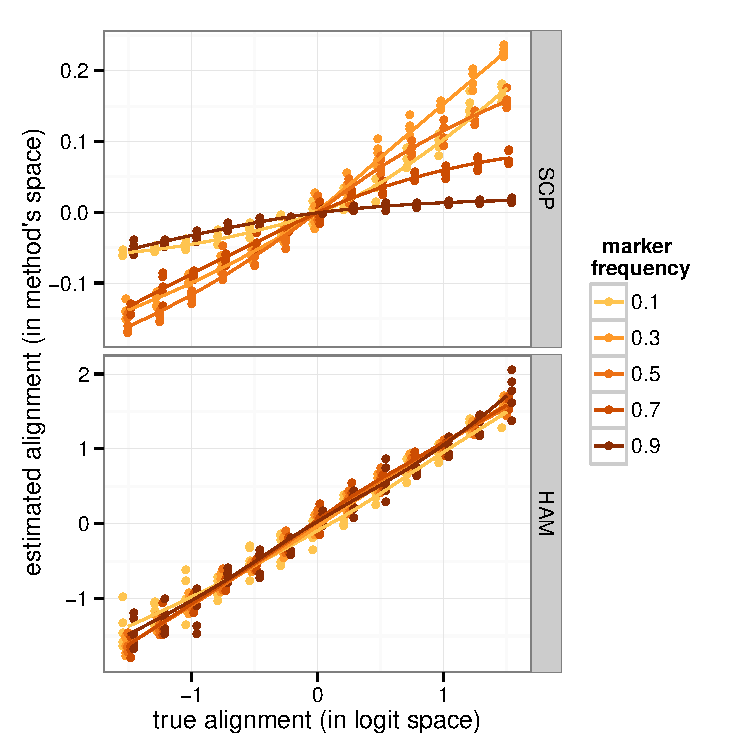
\includegraphics[width=\columnwidth]{graphics/www2016_simulation1_crossiter.pdf}
\caption{Results from simulation 1. Plot shows the actual alignment values from the simulations against the model-inferred values of the alignment. Lines are loess-fit curves. The SCP measures show substantial influence of the marker's baseline probability; the HAM measures are consistent across a range of alignments.}\label{fig:sim1}
\end{figure}

Figure \ref{fig:sim1} shows alignment values recovered by SCP and HAM measures. SCP shows a decreasing slope as the marker baseline frequency increases.  Additionally, within a given baseline frequency, the relationship between true and estimated alignment is non-linear, especially at high or low marker frequencies and alignments. Both of these indicate substantial bias in the SCP measure based on frequency and alignment. In contrast, HAM shows a linear relationship between true and estimated alignment, and the slope of the true-estimated alignment relationship is consistent across different marker frequencies.  Thus, HAM (but not SCP) satisfies the marker frequency consistency and is robust in its estimates from sparse data.

\subsection{Simulation 2: By-word Generation}

Our second simulation uses a slightly more complex generative process, first generating a length for a message and then filling in words within the message. This process moves closer to the true generative process underlying person-to-person conversation; because it generates full messages it also allows testing of the LLA and LSM measures.

We again start by generating $500$ interacting dyads, exchanging a mean of $5$ message pairs. The number of words in each message is drawn from a uniform distribution on the interval $[1,25]$, approximating the 140-character limit of Twitter. We specify a unigram probability $p$ for the marker. The first message in each pair is generated with this unigram probability.  If the initial message does not contain the marker, the reply is also generated with unigram marker probability $p$. If the initial message does contain the marker, the reply marker unigram probability is changed by $\alpha$ in log-odds space.  We vary the marker frequencies over a range representative of common words ($.005 \approx by$, $.01 \approx that$, $.05 \approx the$ in \cite{Brown}) or word categories ($.1 \approx $ personal pronouns, $.2 \approx $ all pronouns, in \cite{KacewiczEtAl2013}), appropriate comparisons for the marker categories used in the Twitter experiments.

Figure \ref{fig:sim2} shows the relationship between true and estimated alignments over the four measures. As in the earlier simulations, the DNM measure is positively correlated with true alignment, but the relationship is somewhat non-linear and dependent on the marker frequency.  With conditionality but no baselining, LLA is able to detect changes in (positive) alignment strength, but is greatly affected by a marker's baseline frequency, as expected. In contrast, LSM fails to correctly capture alignment in this simulation, detecting the greatest ``alignment'' when there is \emph{no} simulated alignment. Since speakers in this simulated dataset all have the same baseline marker frequencies, if they speak independently of each other, their rate of marker usage will be approximately the same. If the replier conditions their marker use on the initial speaker, the replier's rate of marker usage will move \emph{away} from that of the speaker, reducing LSM.  This simulation thus shows that LSM actually quantifies the homophily of a dyad, rather than the alignment---providing evidence that the conditionality/baseline desideratum is critical for separating out alignment from homophily. HAM performs best, showing consistency across markers and robustness in getting accurate estimates from sparse data. 

\begin{figure}[t]
\centering
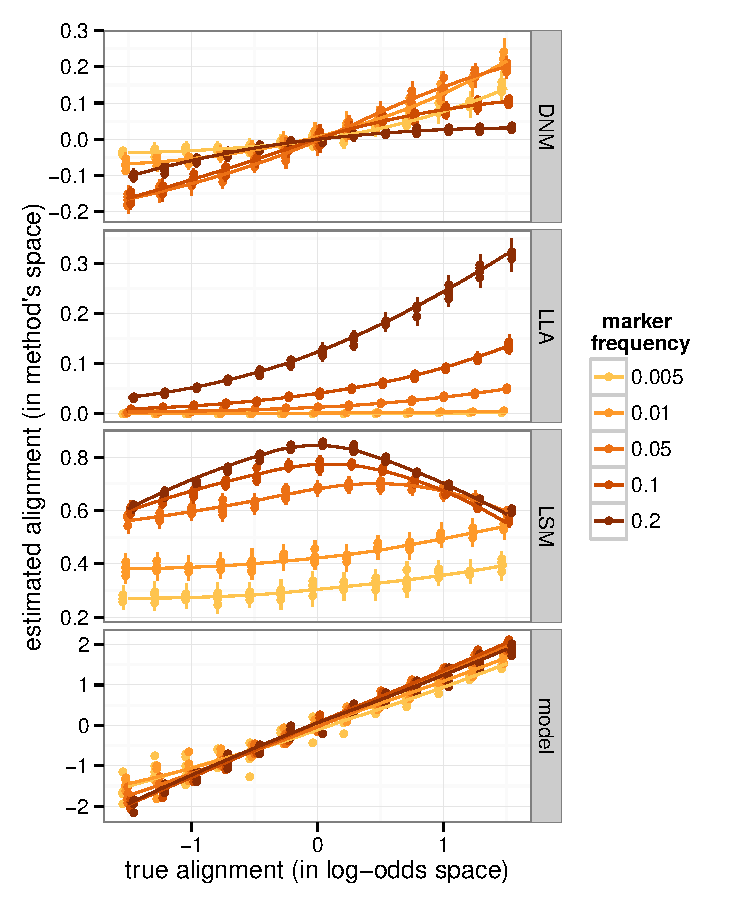
\includegraphics[width=\columnwidth]{graphics/www2016_simulation2b_crossiter.pdf}
\caption{Results from simulation 2. Plot shows the actual alignment values from the simulations against the model-inferred values of the alignment. Ranges shown are bootstrapped 95\% confidence intervals over different simulation runs; lines are loess-fit curves.}\label{fig:sim2}
\end{figure}


%\begin{figure*}
%\centering
%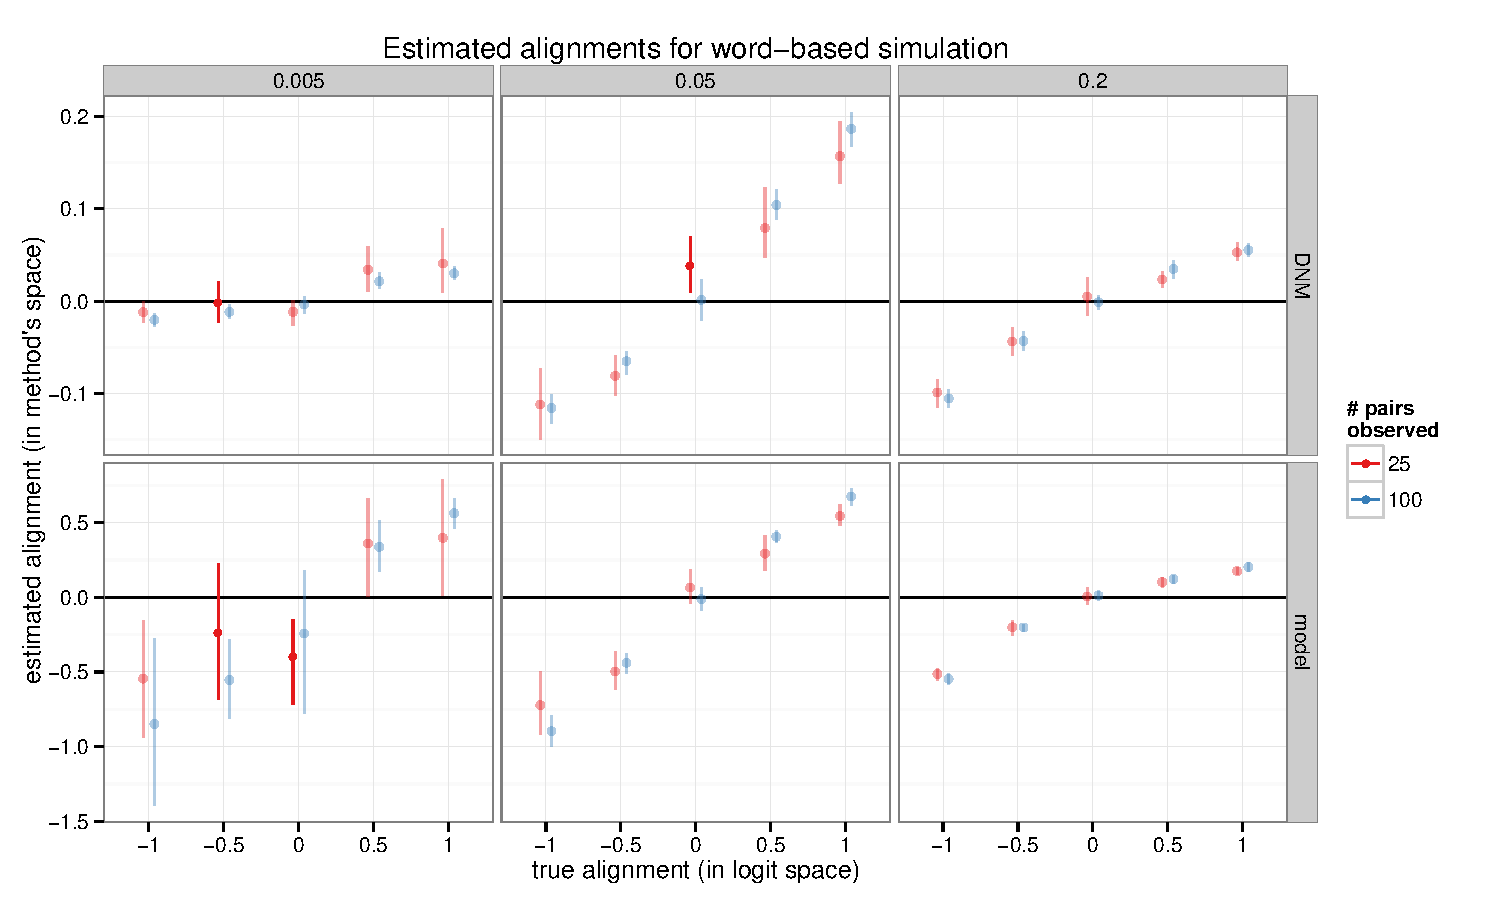
\includegraphics[width=.9\textwidth]{graphics/www2016_simulation2_simple.pdf}\label{fig:sim2}
%\caption{Results from simulation 2. Rows are different alignment measures; columns different baseline word frequencies.  Ranges shown are bootstrapped 95\% confidence intervals over different simulation runs. Opaque parameters indicate false positives or false negatives.}
%\end{figure*}


\section{Experiment 2: Twitter Data}

We next turn to an examination of alignment on Twitter. Because of its size, the diversity of its userbase, and the public accessibility of its data, Twitter is an important source of data about naturalistic linguistic interaction that overcomes many of the limitations of other more restricted sources. On the other hand, as noted above, the brevity of tweets and the sparsity of individual interactions pose substantial challenges to investigators. 

Alignment on Twitter was initially investigated by \cite{DNMGamonDumais2011}, who found overall positive alignment on all 14 marker categories, but no significant effects of social power/status on alignment. This null finding was contrary to findings of power/status effects in many other settings \cite{Gnisci2005}, including some Web-based settings \cite{DNMEtAl2012,NobleFernandez2015}. While it is possible that social media does not display power/status-based differences in alignment -- perhaps because status differences are less obvious in the social media setting -- it is also possible that differences in that earlier study were masked by precisely the problems we highlight above, namely sparse data and widely varying baseline marker frequencies. Using the HAM model we provide evidence for this latter possibility.

\subsection{Corpus}

We use a collection of Twitter conversations collected by \cite{DoyleFrank2015CMCL} to examine information density in conversation. This corpus focuses on conversations within a set of 14 mostly distinct subcommunities on Twitter.  These subcommunities contain all the messages exchanged between Twitter users who sent at least one message to a ``seed user'' with a reasonably large number of followers. This corpus contains 63,673 conversation threads, covering 228,923 total tweets.  We divide these conversations into message pairs, also called conversational turns, which are two consecutive tweets within a conversation thread.  The second tweet is always an explicit reply to the first, and the two tweeters in the pair must be distinct users (i.e., no self replies are included).  

One additional piece of processing is done: while formal retweets (sharing another tweeter's message to one's own timeline) are removed from the data automatically, there are a variety of informal retweeting methods that are not marked by the Twitter API.  We therefore removed all pairs where the reply tweet contained all of the words of its preceding tweet and additionally had either the bigram \textit{RT @username:} (indicative of a ``manual retweet'') or Unicode curly quote characters (indicative of a type of quoting that some Twitter apps use).  In these cases, the entirety of the previous message was included, ensuring maximal alignment, but the words were provided as repetition of a quote rather than being produced as part of the replier's message.  This leaves us with 122,693 message pairs, spanning 2,815 users.

The tweets were parsed into word tokens using the Twokenizer \cite{OwoputiEtAl2013}, with usernames and URLs removed.  We then calculated linguistic alignment on the fourteen marker categories used by \cite{DNMGamonDumais2011} in their study of Twitter messages.  These categories come from the Linguistic Inquiry and Word Count (LIWC) system \cite{LIWC}; category names and sample words are shown in Table \ref{tab:LIWC}. These categories were chosen (from the complete set of 74 LIWC categories) as ``strictly non-topical style dimensions'' as they had limited to no content words in them, and were not focused on specific topics.  These can be roughly divided into four pronoun categories (indefinite, 1st singular, 1st plural, 2nd), four other syntactic categories (article, conjunction, preposition, quantifier), and six conceptual categories (certainty, discrepancy, exclusive, inclusive, negation, tentative).

A tweet is counted as containing a given category if it contains at least one word from that category.  Alignment is calculated based on category rather than on specific word types; thus if the first tweet contains \textit{an} and its reply contains \textit{the}, this pair is counted as an example of positive alignment.

\begin{table}
\centering
\caption{Marker categories for linguistic alignment, with examples, number of distinct word types, and probability of appearing in a tweet.}\label{tab:LIWC}
\begin{tabular}{|c|c|c|c|} \hline
Category & Examples & Size & $p(A)$\\ \hline
Article & \textit{a, an, the} & 3 & .44 \\
Certainty  & \textit{always, never} & 83 & .18 \\
Conjunction  & \textit{but, and, though} & 28 & .39\\
Discrepancy  & \textit{should, would} & 76 & .20 \\
Exclusive  & \textit{without, exclude} & 17 & .27\\
Inclusive  & \textit{with, include} & 18 & .30\\
Indefinite pronoun  & \textit{it, those} & 46 & .39\\
Negation  & \textit{not, never} & 57 & .21\\
Preposition  & \textit{to, in, by, from} & 60 & .58\\
Quantifier  & \textit{few, many} & 89 & .26\\
Tentative & \textit{maybe, perhaps} & 155 & .23\\
1st person singular  & \textit{I, me, mine} & 12 & .57\\
1st person plural & \textit{we, us, ours} & 12 & .14\\
2nd person pronoun   & \textit{you, yourself} & 20 & .25\\
\hline\end{tabular}
\end{table}

\subsection{Overall Alignment}

\cite{DNMGamonDumais2011} found significant positive alignment on all fourteen marker categories on Twitter, but did not detect an effect of power on alignment.  We start by replicating the overall positive alignment result before moving on to the effects of power.  Figure \ref{fig:overall-alignment} shows the alignment values for this Twitter dataset using the measure from \cite{DNMGamonDumais2011} on the left, and our model-based alignment measure on the right.  95\% confidence intervals are shown, based on 1000-draw bootstrapping. [TODO: fix description of error bars] As expected, both measures find consistent and significant convergent alignment on all fourteen marker categories.  

\begin{figure}[t]
\centering
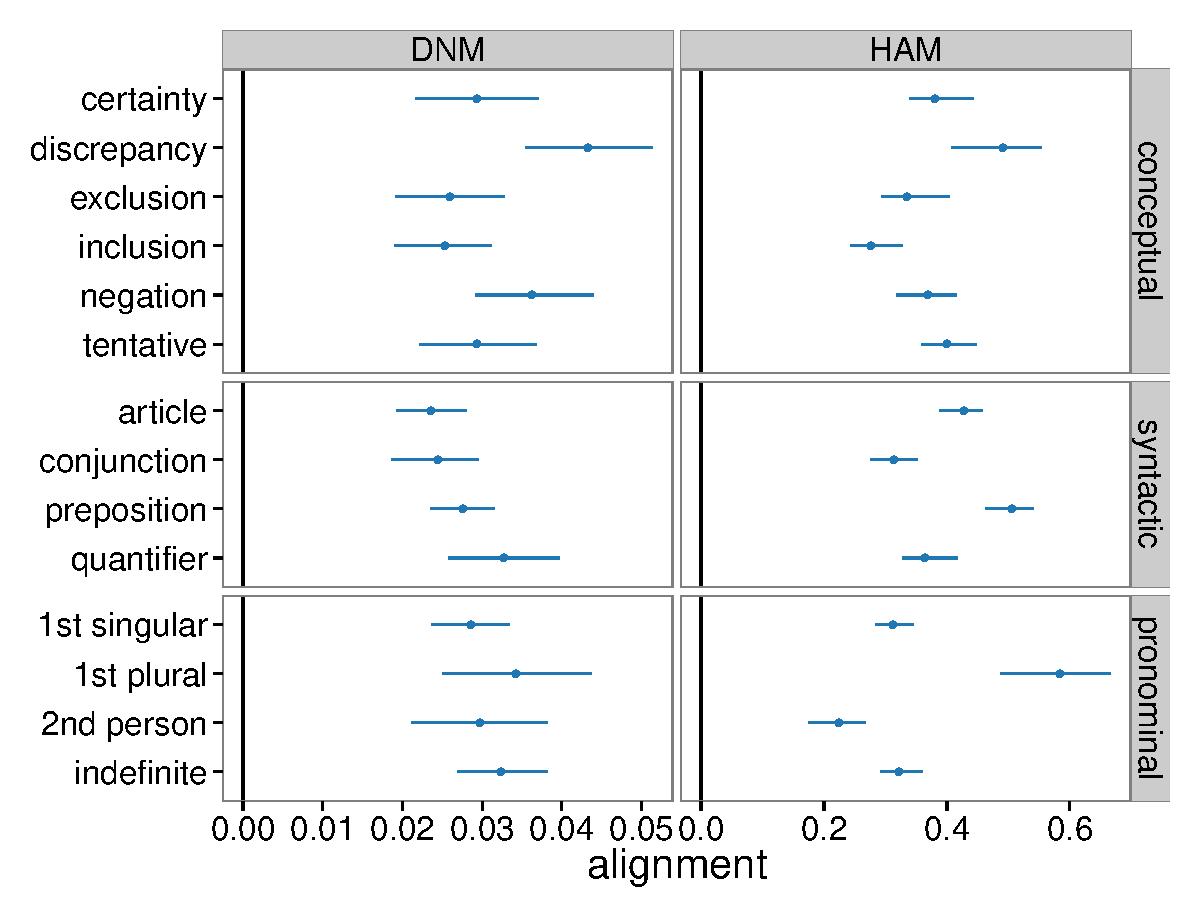
\includegraphics[width=.9\columnwidth]{graphics/www2016_alignmentdnmour_final95.pdf}
\caption{Overall alignment per marker category for SCP and HAM alignment. All 14 marker categories show significant convergent alignment. 95\% confidence intervals shown, based on by-dyad bootstrapping for SCP and by-iteration parameter estimates for HAM.}\label{fig:overall-alignment}
\end{figure}

[TODO: talk here about differences in category behaviors, or save it for power subsection?]

\subsection{Alignment and Power}
% commented this out because it's redundant with above. 
% We are especially interested in applying the model-based measure to the specific question of whether power influences the strength of alignment, as has been shown in other settings \cite{DNMEtAl2012,NobleFernandez2015}. Previous work \cite{DNMGamonDumais2011} showed that Twitter users do align to each other on average, but did not show increased alignment to power.  We expect that the improved sensitivity of our model-based alignment measure will show the anticipated effect of alignment to power.

We assess a user's power on Twitter in two ways. First, we assess power internal to the Twitter network based on the number of other users following our user of interest.  Users with more followers have their tweets read by more users, get more retweets and favorites, and so on, lending them power within the network.  In addition, if they retweet or reply to another user, it can substantially increase that user's status and follower count.  Second, we take advantage of Twitter's user verification process as an external measure of power.  Twitter verifies important users to show that their accounts are not impostors or parodies.  Verified accounts range from heads of state (\texttt{@POTUS, @MedvedevRussiaE}) to famous athletes (\texttt{@KingJames,@Shaq}) to Youtube stars (\texttt{@camerondallas,@pewdiepie}). Twitter only verifies users who they consider to be significant, generally for accomplishments outside of Twitter (though the service does not provide a public standard for verification).  We expect these to measures of power to behave similarly; both verified users and users with high follower counts will be aligned to more than unverified users and users with small follower counts.

Intuitively, alignment to power captures the idea that we show deference to important people that we do not show to our friends. While increased alignment to the power has been observed in many non-Web settings (e.g., \cite{guo2015}), it is possible that the different dynamics of social media would remove or even reverse this effect.  Trolls, cranks, and a variety of other non-cooperative conversationalists may fill people's Twitter timelines (some celebrities and athletes leave or avoid Twitter for this reason). We predict that social media is not so different from other settings, however, and that a sufficiently sensitive measure should find an effect of power.

\subsubsection{Follower ratio as a measure of power} 

For each pair of users, we calculate their \textit{follower ratio} by dividing the first tweeter's follower count by the sum of their follower count and their replier's follower count.  Numbers above 0.5 indicate that the first tweeter has more followers than the replier.  We use $100/101$ as our cutoff, meaning that the first tweeter has at least 100 times as many followers as the replier, and thus has a substantially larger audience. 38\% of our pairs have this property.  Under the hypothesis of increased alignment to power, we expect to find increased alignment when the follower ratio is high.\footnote{We repeated all of these analyses using the median follower ratio, $.9$, as the cutoff, and found no substantive differences between these two cutoffs.}

% [TODO: note that we do not separately look at low speaker follower count ratios, because high follower count people very rarely talk enough to low follower count people to assess alignment.]


\begin{figure}[t]
\centering
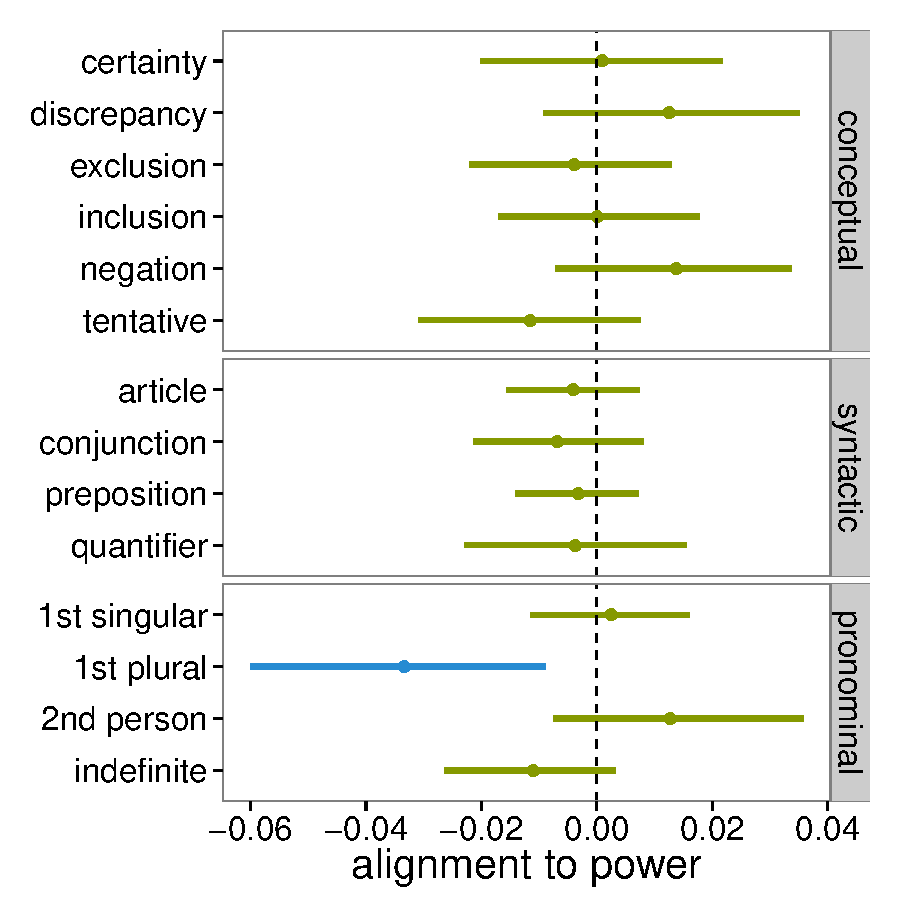
\includegraphics[width=.9\columnwidth]{graphics/www2016_dnmpowerdiff_fratio_final.pdf}
\caption{Difference in SCP-estimated alignment on the 14 marker categories depending on follower ratio. Positive values indicate greater alignment to high-follower users; negative indicates greater alignment to low- and equal-follower users. One category, first-person plural pronouns, shows a significant \textit{negative} effect of power on alignment, while the rest show no effect.}\label{fig:dnm-fratio}
\end{figure}

Figure \ref{fig:dnm-fratio} shows the difference in alignment to power derived from follower counts, using the SCP measure. Here one category shows a significant \emph{negative} effect of power on alignment -- first-person plurals, which, like the second-person pronouns in the verification-power experiments, may have different usage patterns for those with and without power.  The rest of the categories show no significant effects.  This result replicates the lack of significant alignment to power found by \cite{DNMGamonDumais2011}.

\begin{figure}[t]
\centering
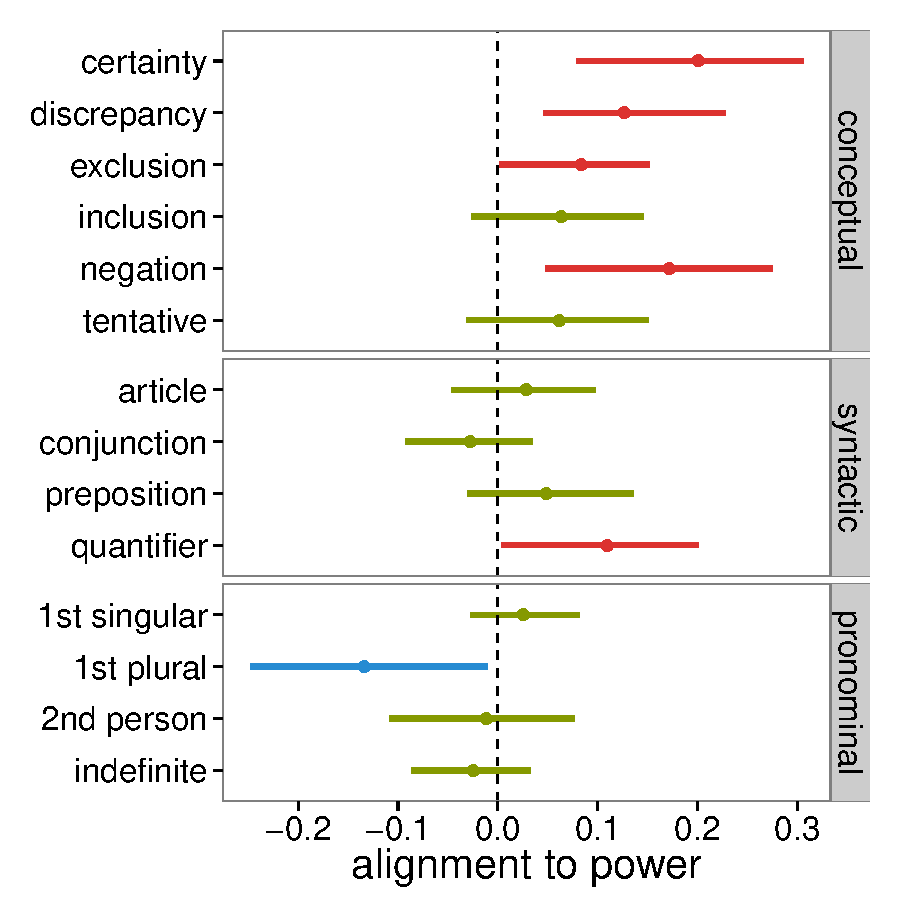
\includegraphics[width=.9\columnwidth]{graphics/www2016_ourpowerdiff_fratio_final95.pdf}
\caption{Difference in HAM-estimated alignment on the 14 marker categories depending on follower ratio. Ten markers show significantly more alignment to power; three of the four that do not are pronouns.}\label{fig:our-fratio}
\end{figure}

Figure \ref{fig:our-fratio} shows the alignment differences based on power derived from follower counts, using our model-based measure.  As with the verification-based power, we see significantly more alignment to powerful users in most categories. First-person plural pronouns are an outlier by this measure, as they were according to the SCP measure.  Overall, though, we see significantly higher alignment to power.

\subsubsection{Verification as power} 

We next examine at tweet pairs with a mismatch in verification.  Because there are relatively few verified users, there were few verified reply tweets in our dataset, and especially few tweets from verified users to other verified users. We focus instead on how unverified repliers adjust their alignment depending on the verification status of the original tweet's sender.  We predict that tweets sent from an unverified user to a verified user will show greater alignment than tweets sent from an unverified user to a fellow unverified user.  

\begin{figure}[t]
\centering
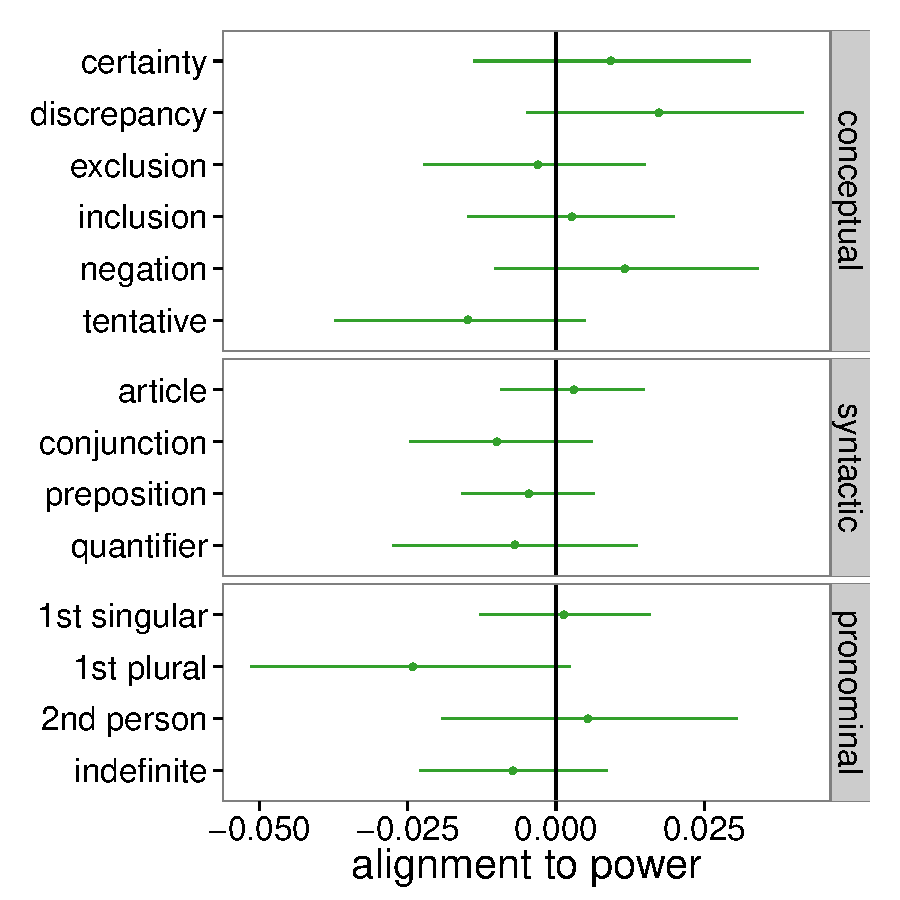
\includegraphics[width=.9\columnwidth]{graphics/www2016_dnmpowerdiff_verif_final.pdf}
\caption{Difference in SCP-estimated alignment on the 14 marker categories when speaking to verified or unverified users. Positive values indicate greater alignment to verified users; negative indicates greater alignment to unverified users. No markers show significant effects of power on alignment.}\label{fig:dnm-verified}
\end{figure}

Figure \ref{fig:dnm-verified} shows the mean difference in per-category alignments when unverified users reply to verified versus unverified users, according to the SCP measure.  A positive value indicates increased alignment to the verified, powerful tweeters.  However, none of the marker categories show significant increases in alignment to verified users, based on the 95\% confidence intervals from a 1000-sample bootstrap.  This replicates the result in \cite{DNMGamonDumais2011}, using their measure.

\begin{figure}[t]
\centering
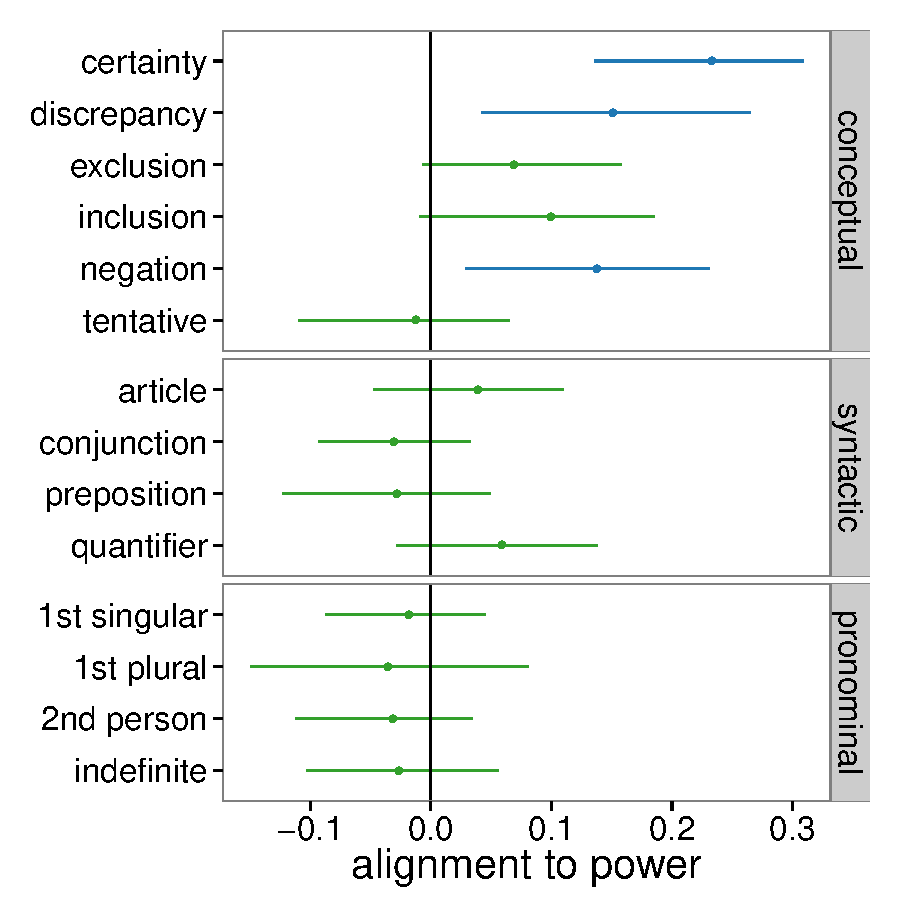
\includegraphics[width=.9\columnwidth]{graphics/www2016_ourpowerdiff_verif_final95.pdf}
\caption{Difference in HAM-estimated alignment on the 14 marker categories when speaking to verified or unverified users. Positive values indicate greater alignment to verified users; negative indicates greater alignment to unverified users. Seven markers show significantly more alignment to power; only five show significantly less.}\label{fig:our-verified}
\end{figure}

In contrast, Figure \ref{fig:our-verified} shows the difference between alignment to verified and unverified tweeters estimated with HAM. Here we see positive differences, indicating higher alignment to verified tweeters, in more than half of the categories.  The one category that shows a negative difference is the second person pronoun category (e.g, \textit{you, yourself, y'all}), which is not entirely unexpected. Work on power dynamics in language have shown that many personal pronouns are used differently by those with and without power \cite{KacewiczEtAl2013,ChungPennebaker2007}, and as such there may be differences in whether \textit{you}-usage triggers reciprocation between two unverified users, of similar social standing, versus between a powerful and non-powerful person.

In these results, we see substantial evidence for a general increase in alignment to a user with more social power, even if that social power is extrinsic to the social network.  Interestingly, we also find compelling evidence for the non-monolithic nature of linguistic alignment. All of the marker categories showed an overall positive alignment effect (Figure \ref{fig:overall-alignment}), but when we compare differences in how people align to with or without power, the markers show idiosyncratic effects.  One class of markers, the pronouns, have previously been shown to interact with power \cite{KacewiczEtAl2013}, and these consistently show less alignment to power than most other markers. Detecting such patterns is a key reason behind the marker separability desideratum.

\section{Conclusions}

Accommodation to one's conversational partners is a deeply ingrained human characteristic, important for assessing the nature of conversation. Linguistic alignment is an important measure of accommodation, and has been a focus for much previous research. Despite this attention, measures of alignment have varied from study to study and field to field, leading to a large body/ of incommensurable results. In addition, as we show here, many widely-used measures either fail to distinguish alignment from homophily, or else suffer from bias across different baseline probabilities and different levels of accommodation. 

We assessed measures on four desiderata: conditionality/baselining, marker separability, consistency across marker frequencies, and robustness to sparse data.  We also introduced a hierarchical, model-based alignment measure (HAM) and showed that it outperformed previous measures in simulations. In an analysis of twitter data, we also showed that this measure is able to detect differential alignment based on differences in social status that were undetectable using previous measures. 

Making theoretical progress on the psychological mechanisms underlying linguistic alignment and communication accommodation more generally will require a consistent and robust set of empirical measurements. We believe our work here takes a step towards developing the kind of method that will facilitate this kind of consistency. Our measures are relatively straightforward to fit, and they result in measurements with a natural scale that can be compared across different settings (e.g., log odds change). We hope that future work will adopt this probabilistic standard, facilitating a more coherent body of investigations of this intriguing set of phenomena. 

%\end{document}  % This is where a 'short' article might terminate

%ACKNOWLEDGMENTS are optional
%\section{Acknowledgments}


%
% The following two commands are all you need in the
% initial runs of your .tex file to
% produce the bibliography for the citations in your paper.
\clearpage
\bibliographystyle{abbrv}
\bibliography{library}  % sigproc.bib is the name of the Bibliography in this case
% You must have a proper ".bib" file
%  and remember to run:
% latex bibtex latex latex
% to resolve all references
%
% ACM needs 'a single self-contained file'!
%
%APPENDICES are optional
\balancecolumns

\end{document}
